% Your system must have a user manual. Append this to your report (make
% it Appendix A) or bind it separately if it is big. If your system is
% interactive and has a good user interface with context dependent help
% then this can be just a cheat sheet. Discuss the level at which your
% user manual is to be pitched with your client. If your system is to be
% extended then you might want to include a technical API manual.

\subsection{Introduction}
\label{s:introduction}

The purpose of the modified version of RoboViz is to enable the visualisation
of multiple robots in the task environment, as opposed to a single robot. The
number of robots that can be held in a swarm depends on how powerful the system
that is running it.

\subsection{Definitions}
\label{s:definitions}

Robot File - A file that defines a robot and its composition.

Configuration File - File that defines the behaviour of the robots when being
visualised.

Robot FileViewer or Visualiser - The window where the user will be able to view
the robots performing.

\subsection{Installation}
\label{s:installation}
Note that the installation only works for the Linux kernel. Although there are
instructions for MacOS, they do not work and a virtual machine is required if
you are not running Linux.

\begin{enumerate}
    \item There are several prerequisites. You can install them with:

    \texttt{sudo apt-get install libboost-all-dev zlib1g zlib1g-dev libprotobuf-dev}
    \texttt{protobuf-compiler gnuplot libopenscenegraph-dev cmake build-essential libtool}
    \texttt{automake libjansson-dev git libpng-dev}
    \item To clone the roboviz git repository, navigate to the directory where
        you want to store the repository and then run the command:

        \texttt{git clone https://gitlab.cs.uct.ac.za/csc3-capstone-project/roboviz.git}
    \item You will also need to install the Open Dynamics Engine via wget. This
        should be in the same parent directory as roboviz:

        \texttt{wget "https://bitbucket.org/odedevs/ode/downloads/ode-0.16.2.tar.gz"}
        \texttt{tar -zxvf ode-0.16.2.tar.gz}

    \item You will need to configure ODE to use double precision:

        \texttt{cd ode-0.16.2}
        \texttt{./bootstrap}
        \texttt{./configure --enable-double-precision --with-cylinder-cylinder=libccd}
        \texttt{sudo make install -j}
    \item Now that the dependencies are ready, change directory into the
        roboviz project folder:

        \texttt{cd ../roboviz}
    \item The build system used by RoboViz is CMake, and the unit tests are
        automatically compiled. Compile the project with:

        \texttt{cd build \&\& rm -rf *}
        \texttt{cmake -DCMAKE\_BUILD\_TYPE=Release -G"Unix Makefiles" ../src}
        \texttt{time make -j2}
        \texttt{cp -r ../models ./}

    \item  Run the tests from the build folder with:
        \texttt{ctest --verbose}

    \item Still from the build folder, the file viewer can be executed with:

        \texttt{./robogen-file-viewer ../examples/sindiso\_single.json }
        \texttt{        ../examples/sindiso\_conf.txt --debug}
    \item And that's it!
\end{enumerate}

You can run different simulations by editing the file
\texttt{examples/sindiso\_conf.txt}. More details about contributing to the
project can be found in \texttt{CONTRIBUTING.md}. Commandline help can be found
by executing the command:

\texttt{cd build \&\& ./robogen-file-viewer --help}

\subsection{The various files in the project}
\hypertarget{resources}{%
\subsubsection{Resources}\label{resources}}

\begin{itemize}
\item
  \href{https://developers.google.com/protocol-buffers}{protocol
  buffers} are used to allow the Evolution Engine and Simulation Engine
  to communicate
\item
  \href{https://github.com/kripken/emscripten}{emscripten} is something
  which converts CPP code to WebAssembly/JavaScript so that RoboGen can
  run in the user's browser. If something has the
  \texttt{\#ifdef\ EMSCRIPTEN} preprocessor macro, then it's used for
  the WebAssembly/JavaScript version and not the desktop version
\item
  \href{https://github.com/peter-ch/MultiNEAT}{HyperNEAT} is a neural
  network evolution algorithm, and RoboGen provides experimental support
  for it.
\end{itemize}

\hypertarget{evolution-engine-files}{%
\subsubsection{Evolution Engine Files}\label{evolution-engine-files}}

\begin{itemize}
\item
  \texttt{src/Evolver.cpp} : Does the evolving of robots. Is the main
  executable for \texttt{./robogen-evolver}.
\item
  \texttt{src/config}: Handles configuration given to RoboGen. Makes
  heavy use of
  \href{https://www.boost.org/doc/libs/1_77_0/doc/html/program_options/tutorial.html}{boost
  program options} which is something that makes it really easy to take
  input from either the command line or from a configuration file in the
  form of key=value pairs
\item
  \texttt{src/evolution/representation} All the code for describing how
  robots are represented in RoboGen

  \begin{itemize}
  \item
    \texttt{src/evolution/representation/RobotRepresentation} is the
    main component here, and is made up of a
    \texttt{src/evolution/representation/PartRepresentation} and a
    \texttt{src/evolution/representation/NeuralNetworkRepresentation}
  \end{itemize}
\item
  \texttt{src/evolution/enging/Mutator} describes how various operators
  act on the robot representation
\item
  \texttt{src/evolution/engine/Population} is a collection which
  individual robots are organised into.

  \begin{itemize}
  \item
    \texttt{src/evolution/engine/IndividualContainer} This is extended
    by \texttt{Population}
  \end{itemize}
\item
  \texttt{src/evolution/neat} is an experimental port of
  \href{https://github.com/peter-ch/MultiNEAT}{HyperNEAT}, a neural
  network evolution program, although I don't think this file is ever
  used directly. Instead it's accessed via
  \texttt{src/evolution/engine/neat/NeatContainer}
\item
  \texttt{src/evolution/engine/neat/NeatContainer} Contains logic used
  to interface between RoboGen and HyperNEAT.
\end{itemize}

\hypertarget{simulation-engine-files}{%
\subsubsection{Simulation Engine Files}\label{simulation-engine-files}}

The simulation engine is built on top of the
\href{http://www.ode.org/}{Open Dynamics Engine}, and it's recommended
by the maintainers that you be well-versed in ODE before attempting to
modify the RoboGen Simulator.

The simulation engine is usually invoked in one of two ways: 1. Running
\texttt{build/robogen-server} to perform fitness evaluations for the
evolver 2. Running \texttt{build/robogen-file-viewer} to ``play back'' a
robot as specified in a configuration file.

Important source files and descriptions 
\begin{itemize}
    \item \texttt{src/Simulator.cpp}: The file which actually does the
        simulating. It relies on many pieces of code, but is called via
        \texttt{Simulator::runSimulations} in these two programs: 
    \item \texttt{src/RobogenServer.cpp}: Used when the evolver wants
        to perform a fitness evaluation of a certain robot, called via
        \texttt{build/robogen-server} 
    \item \texttt{src/viewer/FileFiewer.cpp}: Used by a person to view a robot
        and watch it move in the task environment.  Called via
        \texttt{build/robogen-file-viewer} 
    \item \texttt{src/model/} contains physical models of robots parts,
        obstacles, light sources, and any other physical items in the task
        environment. 
    \item \texttt{src/model/components/} contains descriptions of the various
        components (Hinges, Actuated components, Passive components, Bricks,
        etc) 
    \item \texttt{src/model/sensors/} Contains descriptions of AMU sensors,
        light sensors, touch sensors, sensor groups, etc 
    \item  \texttt{src/model/motors/} Describes general motors and servo motors. 
    \item  \texttt{src/model/objects/} Describes light sources and obstacles 
    \item  \texttt{src/render/components/} Has renderer friendly versions of
        every model in RoboGen. Note that when the \texttt{robogen-file-viewer}
        is run, you do \emph{not} see the physical model of the robot as the
        evolver sees it. You see a representation of how the robot will look
        when 3D printed, but the evolution algorithm sees a bunch of connected
        primitive blocks (cubes, joints, planes, etc) which have much less
        detail than the 3D printed parts, although should function the same
\end{itemize}

\hypertarget{other-files}{%
\subsubsection{Other files}\label{other-files}}

\begin{itemize}
\item
  \texttt{src/robogen.proto} Defines what the protocol buffers look
  like, and is automatically converted to CPP code by the
  \href{https://developers.google.com/protocol-buffers/docs/cpptutorial}{protobuf}
  compiler.
\item
  \texttt{src/utils/network/} Contains most of the code for socket-based
  communication between programs.
\item
  \texttt{src/utils/json2pb} Is used for converting protobuf messages
  to/from json (since json is used when we want to save an individual
  robot)
\item
  \texttt{src/arduino/} contains files for generating a
  \texttt{NeuralNetwork.h} file for use on Arduino.
\end{itemize}

\subsection{Running RoboViz}
\label{s:runningroboviz}

To start viewing the robot in the task environment, you'll need to enter the
commands displayed in the pictures below.
\begin{figure}[htpb]
    \centering
    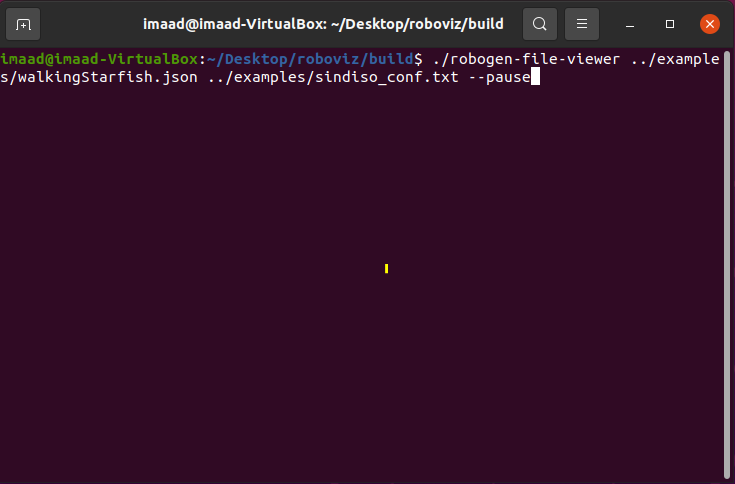
\includegraphics[width=0.8\textwidth]{run}
    \caption{commands in terminal }
    \label{fig:commands-in-terminal}
\end{figure}

Once entered, the screen shown in Figure \ref{fig:robots-in-visualiser} should
be displayed.
\begin{figure}[htpb]
    \centering
    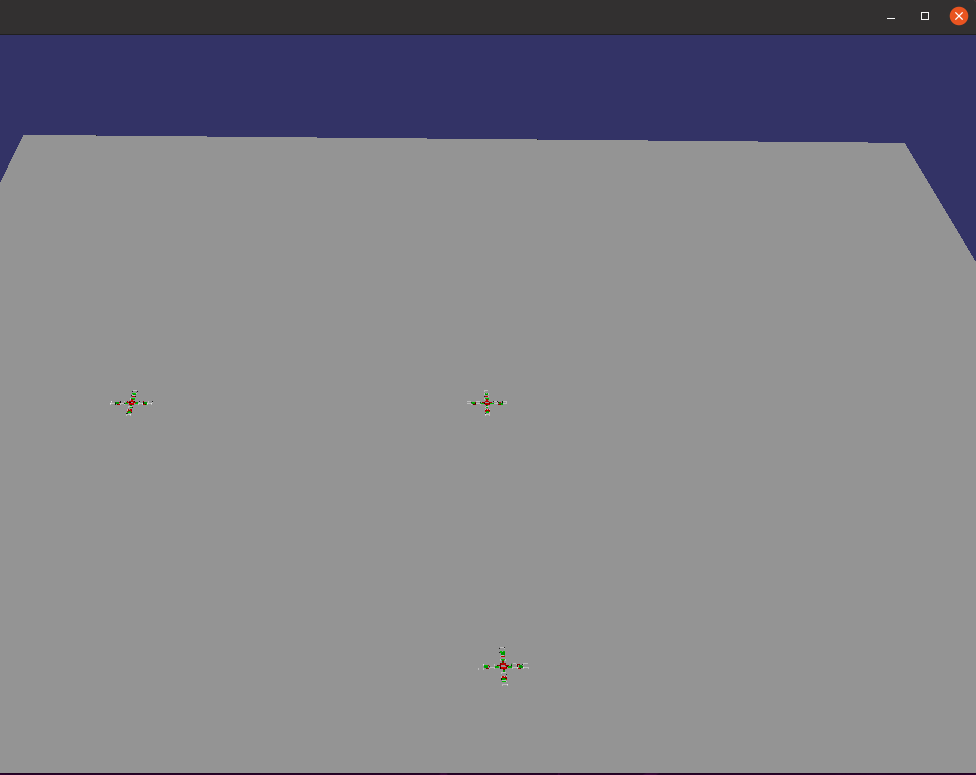
\includegraphics[width=0.8\textwidth]{visual1}
    \caption{Robots in Visualiser}
    \label{fig:robots-in-visualiser}
\end{figure}

